\chapter{Design}
\section{Overview}
This section covers the complete development process including the hardware, gateware, software and mechanical design of the project. Important to note is, that the following documentation concentrates only on the final version of the device. Earlier hardware prototypes are not covered due to the lack of relevance.

\subsection{Key Requirements}
The main focus of the development is to design a professional looking, easy to use and eye-catching device for demonstration purposes such as info days. The project name \textit{Audio-Beamformer} has been chosen as it is easy to remember and has potential to be seen as a trademark. 

The following key requirements have been set:
\begin{itemize}
    \item Single power adapter or power cable (e.g. no need of labor power supplies) 
    \item Easy to install (e.g. montage on a camera tripod)
    \item Intuitive to operate via state-of-the-art graphical user interface
    \item Multiple audio streaming sources such as Bluetooth and USB input devices
    \item Great scalability and flexibility of the hardware and software design
\end{itemize}

\subsection{Key Decisions}
In the conceptional phase of the development, several key decisions had to be felt. This contains mainly the signal flow and the division between the processing part on the Raspberry Pi and the \acrshort{fpga}. Further, the question had to be evaluated, if a built-in power supply or an external power adapter is preferred. And most importantly, which type of ultrasonic transducer should be used in the design.
In addition, the overall dimension and scale of the final product had to be discussed. 
In general, most of these decisions were felt by the result of simulations, physical measurements and after extensive discussions.
In the following sections, each part of the project is explained in more detail.


\newpage
\section{Hardware Design}
The hardware of the Audio-Beamformer was designed using Altium Designer 22. The integrated 3D \acrshort{cad} functionality simplified the overall development and lowered the possibility of errors in the design.
The hardware has been improved over several iterations until a final version could be built.\\
The 2-Layer \acrfull{pcb} with the size of 300.0\,mm\;x\;376.0\,mm has been manufactured and assembled by JLCPCB.\\

\begin{figure}[h!]
	\centering
	\includegraphics[width=14cm]{images/4_Design/Hardware/Audio-Beamformer_PCB.jpg}
	\vspace{-0.2cm}
    \caption{3D-Render of \acrshort{pcb}}
    \label{fig:pcb_render}
\end{figure}
\newpage

\subsection{Block Diagram}
\begin{figure}[h!]
	\centering
	\includegraphics[width=21.5cm, angle=90]{images/4_Design/Hardware/System Block Diagram 2.pdf}
	\vspace{-0.2cm}
    \caption{System Block Diagram}
    \label{fig:hardware-block-diagram}
\end{figure}

\clearpage
\subsection{Power Management}
The Audio-Beamformer is powered directly by mains voltage. As a connector, the widely used C14 (IEC 60320) has been chosen. Because of the metallic casing, protective earth is required. It has been connected directly to the back panel. The main switched mode power supply is made by \textit{Mean Well} and delivers 48\,V \acrshort{dc} and up to 163\,W output power. The LSP-Series is specially designed for low-profile applications and therefore ideal in this use case.\newline
The simplified power management diagram \ref{fig:simplified-power} provides a better overview of how each voltage rail is created.

\begin{figure}[h!]
	\centering
	\includegraphics[width=\textwidth]{images/4_Design/Hardware/Power Supply Overview.pdf}
	\vspace{-0.6cm}
    \caption{Simplified Power Management}
    \label{fig:simplified-power}
\end{figure}

As a reversed polarity protection a schottky diode has been placed directly after the input connector. Further \acrshort{dc}-\acrshort{dc} buck converters generate fixed 5\,V (6.5\,A), 12\,V (2.0\,A) and a variable HV rail.


\bigskip
\begin{wrapfigure}{r}{7cm}
    \vspace{-0.6cm}
    \includegraphics[width=7cm]{images/4_Design/Hardware/Variable Buck-Converter.pdf}
    \vspace{-0.6cm}
    \caption{Variable Buck-Converter}
    \label{fig:variable-buck-converter}
\end{wrapfigure} 
For adjusting the physical output volume of the ultrasonic transducers, the amplifier drive voltage must be changed accordingly. The HV voltage supply can be set between 5.2\,V and 23.5\,V (2.0\,A). This has been achieved by using a digital potentiometer (MCP41010T) which is controlled by an \acrshort{spi}-Interface.\\
For safety reasons, the HV voltage is turned off per default and must be enabled by a physical logic signal provided by the Raspberry Pi.
\clearpage

The output voltage can be calculated as follows

\begin{equation}
    V_{HV}(R_{var}) = \frac{V_{ref}}{R_{bot} + R_{var}} (R_{bot} + R_{top} + R_{var}).
\end{equation}

Where $R_{var}$ is proportional to its 8-bit value (\codeword{0x00} $\cong$ 0\,$\Omega$ and \codeword{0xFF} $\cong$ 10\,k$\Omega$). The reference voltage of the DC-DC buck converter (LM2596HV) is 1.23\,V. The resistor values used in the design are $R_{top}$ = 39\,k$\Omega$, $R_{bot}$ = 2.0\,k$\Omega$ and $R_{var}$ = 10\,k$\Omega$. This leads to the following approximation
 \begin{equation}
    V_{HV}(d) \approx 5.2\,V + d\:\frac{20\,V}{255}.
\end{equation}

\subsection{Raspberry Pi Compute Module 4}
As a main processing platform the Raspberry Pi Compute Module 4 has been chosen due to its powerful quad-core processor and the great software support based on a large community. The exact model used in the design has 4\,GB of \acrshort{ram} and fixed installed 16\,GB of embedded \acrshort{emmc} flash storage. This has the advantage of being more reliable than systems that are dependent on a \acrshort{sd}-Card.
To increase the performance, the Raspberry Pi has been overclocked to 1.0\,GHz. Sufficient cooling is provided by a heat sink and four cooling fans.
The \acrshort{io} operating voltage has been set to 3.3\,V.

\subsection{FPGA} \label{hardware_fpga}
There are two \acrshort{fpga}s used in the design for generating the drive signals for the ultrasonic transducers. Each \acrshort{fpga} is mounted on a development board called \textit{Alchitry Cu}. They are installed as daughter-boards on the main \acrshort{pcb} by high-speed board-to-board connectors. Both \acrshort{fpga}s receive the audio stream via an \acrshort{i2s}-Stream and get controlled by a simple \acrshort{spi}-Protocol in an daisy-chain configuration. More details on this in section \ref{fpga_i2s} and \ref{fpga_spi}.\\
The \acrshort{fpga} boards are powered by 5\,V, because they have an on-board 3.3\,V regulator build-in.


\subsection{Sensors and HMI}
The Audio-Beamformer contains several sensors that are connected by different interfaces to the Raspberry Pi Compute Module. The \acrfull{hmi} enables easy access to change various settings of the device.

\subsubsection{Camera}
To be able to direct the sound towards a specific person, a camera is needed. In this case a \acrshort{usb}-Camera has been chosen since it is easy to connect and does not need any special device drivers. The type \textit{ELP-USB500W02} provides a resolution of 1280\,x\,720 pixels and a frame rate of up to 30\,FPS. The optics used in this application are designed to match the viewing angle of the camera to the maximal beam-steering angle of the Audio-Beamformer. In this particular case, a camera lens with a focal length of 4.2\,mm has been chosen which results in a viewing angle of ca. ±40°.

However the camera had to be slightly modified. On startup, it tries immediately to establish an \acrshort{usb} connection to the host device. If there is no response during the first 500\,ms the camera goes into a power-down/suspend mode. In this state it can't be recognized by the host until it gets power-cycled. This issue has been solved by increasing the RC time constant of the camera internal power-on reset circuitry from 4.7\,ms to ca. 4.7\,s. In addition a schottky diode has been added to guarantee a fast discharge time after powering off the device. This ensures a valid reset-pulse even if the device gets power-cycled very rapidly.

\begin{figure}[h!]
    \centering
    \subfloat[\centering Reset-Circuit]{{\includegraphics[height=6cm]{images/4_Design/Hardware/Camera Reset-Circuit.pdf}}}
    \qquad
    \subfloat[\centering Location of RC-Circuit]{{\includegraphics[height=5.5cm]{images/4_Design/Hardware/Camera-Modification.PNG}}}
    \caption{Camera Modification}
    \label{fig:camera-modification}
\end{figure}


\subsubsection{Temperature Sensor}
There are two temperature sensors embedded on the \acrshort{pcb}. One to measure the ambient temperature (and therefore be able to calculate the speed of sound in air according to the temperature, described in \ref{equ:speed_of_sound}) and the second-one to measure the system temperature which is used to control the speed of the four \acrshort{dc}-Fans. The temperature sensors used in the design are of the type \textit{TMP112} made by Texas Instruments. They have an accuracy of ±0.5\,°C and are connected to the \acrshort{i2c}-Bus of the system with individual IDs (\codeword{0x48} \& \codeword{0x49}). The temperature gets read every 500\,ms.

\subsubsection{Time-of-Flight Sensor}
For various safety reasons it is important to turn off the speaker output when a person enters the near-field of the Audio-Beamformer (d $<$ 1\,m). This safety mechanism has been realized by using a multi-zone \acrfull{tof} sensor. The \textit{VL53L5CX}, made by ST Microelectronics is specially designed for a wide field of view (63°). It can measure distances up to 4\,m and has a resolution of 8\,x\,8 zones. It is connected to the \acrshort{i2c}-Bus and can be address by the ID of \codeword{0x52}. The internal update rate has been set to 5\,Hz to minimize traffic on the \acrshort{i2c}-Bus. To further increase the data throughput, the \acrshort{i2c} clock rate has been set to 1\,MHz.

The distance-map data then gets further processed as described in section \ref{4_Sensors_Near-field}.

\newpage
\subsubsection{Rotary Encoder}
To easily adjust the volume of the Audio-Beamformer, a pushable rotary encoder has been placed below the display. Pressing the knob toggles the mute state of the output stage. This becomes very handy if the volume level should stay the same, but the speaker needs to be turned off temporarily. Both, the volume level and the mute state can be overwritten in the \acrshort{gui}. This is can only be achieved by the relative position measurement of rotary encoders and would not be possible with ordinary potentiometers.

To suppress contact bouncing and thus prevent false inputs, a simple RC debouncing circuit with a schmitt-trigger buffer has been installed.

\begin{figure}[h!]
	\centering
	\includegraphics[width=8.5cm]{images/4_Design/Hardware/Rotary Encoder Debounce.pdf}
	\vspace{-0.1cm}
    \caption{Rotary Encoder Debounce-Circuit}
    \label{fig:rotary_encoder-debounce_circuit}
\end{figure}

\subsubsection{Power-Button and Cooling-Fans}
On the right side of the Audio-Beamformer, a 22\,mm stainless steel push button has been installed to power-on and off the Raspberry Pi Compute Module 4. The integrated \acrshort{rgb}-\acrshort{led} ring is driven by a specialized \acrshort{pwm}-Driver \acrshort{ic} with \acrshort{i2c}-Interface. The \textit{PCA9633DP1}, made by Texas Instruments provides four individual addressable 8-Bit \acrshort{pwm} channels and is addresses at the \acrshort{i2c}-Address of \codeword{0x62}. \acrshort{pwm}-Channel 1, 2 and 3 are used for the red, green and blue \acrshort{led}s of the bush button, while channel 0 is connected to the four \acrshort{dc}-Fans installed in the back of the enclosure. The Fans are wired in parallel and operate at a maximal voltage of 12\,V.\\
The system temperature is used to control the speed of the cooling fans. They start running at a temperature of 40\,°C and provide proportional air flow as the temperature increases. At 60\,°C the operate at full speed.

\subsubsection{LCD Touchscreen}
Since the beginning of the project, the idea was to create an attractive and modern looking device. One of the key components is the large \acrshort{lcd} touchscreen. It has a diagonal size of 11.9\,inch and a resolution of 1480\,x\,320 pixels. As interface, \acrshort{hdmi} is used for the video stream and \acrshort{usb} to transmit the touch-screen data to the Raspberry Pi Compute Module 4. Important to notice is, that the corners of the display are rounded (radius of 5\,mm), this has been considered when designing the \acrlong{ui}.

\subsubsection{RGB-LEDs}
To present a visual feedback of the current beam-steering angle and the active window-function, each row of the array contains one individually addressable \acrshort{rgb}-\acrshort{led} on top and on the bottom of the ultrasonic transducers. The type of those intelligent \acrshort{led}s is called \textit{APA102}. They embed an integrated driver \acrshort{ic} which can be controlled via a non-standard \acrshort{spi} protocol (special start and end sequence instead of a chip select line) in a daisy-chain configuration. The LEDs have a physical size of 5.0\,x\,5.0\,mm and are directly powered by the 5\,V voltage rail.\\
Next to the 38 \acrshort{led}s used for the array channel illumination, further 20 \acrshort{led}s are placed on a ring around the camera. This offers direct visual insight of the face-tracking algorithm. While a person is tracked, the \acrshort{led}s are animated in a "breathing" brightness motion. When there is no face detected, a spinning gradient animation is shown.\\
The maximal power consumption is about 25\,W if all \acrshort{led}s are fully turned on.

\subsubsection{External Interfaces}
The Audio-Beamformer can easily be connected to an external display by using the \acrshort{hdmi}-Port on the left side of the enclosure. In combination with the two spare \acrshort{usb}-Ports, e.g. for connecting a keyboard and mouse, the system can easily be debugged. Even developing new software features directly on the target platform is possible. To back-up the data of the \acrshort{emmc} flash storage on the Raspberry Pi Compute Module 4, a  \acrshort{usb} Type-C Port has been added. To start the back-up procedure, the tiny slide switch next to the \acrshort{usb}-C Port must be set to the up-position. This enables the bootloader of the Raspberry Pi Compute Module 4 on power-up of the device. When connected to an external host (such as a computer), the Audio-Beamformer gets recognized as a mass-storage-device. A back-up tool like e.g. \textit{Win32DiskImager} can be used to create a binary image of the operating system inclusive all user data.

\subsection{Output Stage}
The output stage represents a Class-D design in a \acrshort{mosfet} full-bridge configuration. This topology has the advantage of high efficiency and low part count. However, the proper design of such output amplifiers has its difficulties. Specially when operated at high switching frequencies (3.125\,MHz in this case), transient turn-on and turn-off times must be very short. This can lead to ringing and voltage spikes on the output signal.
\acrshort{mosfet}s are known to be very sensitive when it comes to such transient voltage spikes. Exceeding the maximal Drain-Source voltage will likely result in a breakdown and a permanent short circuit. To prevent such behavior, several options can be considered:

\begin{itemize}
    \item Utilize \acrshort{mosfet}s with higher voltage rating
    \item Reduce switching speed and therefore increase transient time
    \item Impedance matching of load and driving source (e.g. with series resistor)
    \item Introducing passive dampening networks, such as RC-Snubber circuits
    \item Dump excess energy into bypass capacitors using clamping diodes
\end{itemize}
\newpage

\acrshort{mosfet}s with higher Drain-Source voltage ratings have typically more gate capacitance and therefore would lead to a drastically higher switching current. A great compromise has been found with the type \textit{BSS123}, it has a Drain-Source voltage rating of 100\,V and can withstand a continuous current of 200\,mA. The gate capacity is around 32\,pF (at a gate voltage of 12\,V). 

\begin{figure}[h!]
	\centering
	\includegraphics[width=5.5cm]{images/4_Design/Hardware/Class D Snubber.pdf}
	\vspace{-0.2cm}
    \caption{Class-D Half-Bridge with RC-Snubber}
    \label{fig:rc-snubber}
\end{figure}

As mentioned above, RC-Snubber networks can help to suppress voltage spikes by creating a low-impedance path for the current, circling in the low-side of the half-bridge. Figure \ref{fig:rc-snubber} shows how important a sufficient bypass capacitor is to stabilize the high-side. Texas Instruments published a very comprehensive guide on how to design such RC-Snubber networks \cite{ti_class_d_snubber_design}.

The amplified digitally modulated output signal must be low-pass filtered in order to suppress the high frequency switching content. This can easily be achieved by the use of a series inductance. To keep the design symmetrical, on both half-bridge output signals a shielded inductor with an inductance of 220\,$\mu$H has been installed. The inductance value has experimentally be evaluated by trying out different combinations of inductors and switch frequencies compared to the output noise level.
%\pagebreak

\subsection{Ultrasonic-Transducer Array}
Achieving a decent array size is important to get a better directivity, higher output volume and in general greater beam-steering properties. Thus a large amount of ultrasonic transducers is needed. In order to keep the cost down of the project, one of the key criteria was the unit price. Directly ordering by professional suppliers, such as Digikey, Mouser, Farnell, etc. results in very high prices of more than 7\,CHF per piece. This was not acceptable since more than 150 pieces are needed in the final design. Fortunately it was possible to get directly in touch with a manufacturer based in China. The datasheet of the \textit{MA40A16} (attached in the appendix \ref{appendix_ma401a6}) has been studied firmly, with the conclusion that the type is suitable for this project and satisfies all key parameters. The price per unit is only 0.3\,CHF.\\
They operate at a resonant frequency of 40\,kHz and have physical diameter of 16\,mm. Important to notice is, that the metal case makes electrical contact to one of the pins. Thus it's important to leave enough clearance between the transducers to prevent short circuits.

\subsubsection{Arrangement \& Placement}
As prior analysis showed, the denser an array can be built, the better is it's performance. Due to the circular shape of the ultrasonic transducers, the optimal arrangement is a hexagonal pattern. This has some further advantage of creating a smaller horizontal spacing between each row of ca. 14.75\,mm (when a diagonal distance of 17.0\,mm is chosen with a gab of 1\, mm between the transducers). In general, a smaller spacing leads to higher efficiency and a better beam pattern (e.g. less dominant side lobes).\\
The final number of 19 rows has been the result of several considerations. First of all, the row count must be odd, to create a symmetrical design with only one centre row. Further the total width of the array must comply with the maximal manufacturing and assembly size of \acrshort{pcb}s by JLCPCB (max. 480\,x\,320\,mm). And at last, the overall dimension should match the size of the display to create a cleaner visual impression of the final design. At some point, adding more rows to the array will not lead to any further audible improvements. This is mainly caused by the window-function which tends to strongly reduce the gains of the rows at both ends of the array.\\
A row height of 8 has been chosen to create stronger beam-characteristics, specially in the vertical direction. In addition, the parallel wiring of multiple ultrasonic transducers lowers the total impedance, which has the advantage of operating at a lower driving voltage to create the same amount of power.

\bigskip
\begin{figure}[h!]
	\centering
	\includegraphics[width=10.5cm]{images/4_Design/Hardware/Transducer Placement.pdf}
	\vspace{0.2cm}
    \caption{Ultrasonic Transducer Placement}
    \label{fig:transducer-placement}
\end{figure}
\newpage

\section{FPGA Design}
As mentioned in Section \ref{hardware_fpga}, the \textit{Alchitry Cu} \acrshort{fpga}-Board has been used. The specific chip is called \textit{iCE40-HX8K}, made by Lattice Semiconductor. It offers a total of 7680 logic cells, 32 blocks of dual-port \acrshort{ram} (4\,KBit each), two independent \acrshort{pll}s and 79 \acrshort{io}-Pins. It is operated at 100\,MHz which is more than enough for this application.

\begin{figure}[h!]
	\centering
	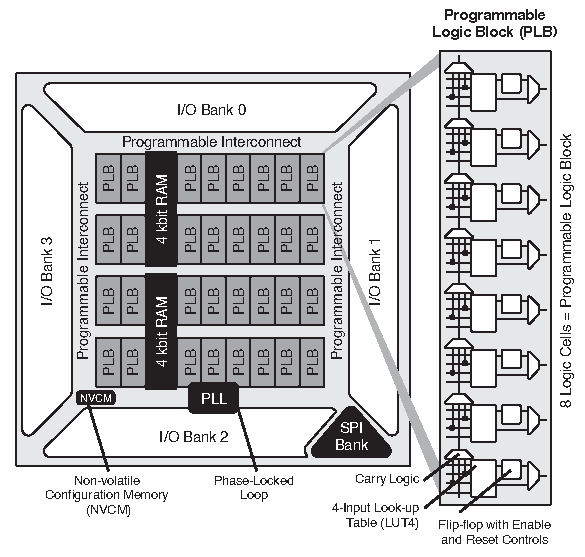
\includegraphics[width=9.5cm]{images/4_Design/FPGA/iCE40LPHXFamilyDataSheet.pdf}
	\vspace{0.0cm}
    \caption{Lattice iCE40 \acrshort{fpga} Family Architecture \cite{lattice_ice40_fpga_architecture}}
    \label{fig:rc-snubber}
\end{figure}

To keep the design process as efficient as possible, a development environment has been chosen which is easy to use and offers lots of predesigned \acrshort{ip}-Blocks. Namely the \mbox{\textit{IceStudio}} has been used in combination with the open source tool-chain called \textit{IceStorm} which currently supports all \acrshort{fpga}s of the iCE40-Family.\\
The tool offers a combination of a graphical design work-flow with the option of embedding custom blocks of Verilog code. Due to the open source nature, lots of individuals published extension libraries containing hundreds of \acrshort{ip}-Blocks. This becomes very handy, specially for integer arithmetic operations, such as addition and multiplication.

\subsection{Integer Arithmetic}
Signed integers with a fixed width of 16 bits have been chosen as a datatype. This has the advantage of making use of dedicated hardware accelerators built into the \acrshort{fpga}. The maximum range of a 16 bit integer reaches from -32,768 to +32,767. In order to make calculations easier, this range can be interpreted as normalized values between -1.0 (representing -32,767) and +1.0 (representing +32.767). Note that the most negative value of -32,768 should never be used, as the same positive value can't be reached (preventing asymmetric behaviour).\\
Using normalized values simplifies particularly the multiplication operation, since signals can be attenuated or mixed without the risk of a sign flip or the values getting clipped.
\newpage

\subsection{Signal Flow Diagram}
\enlargethispage{2.6cm}
\begin{figure}[h!]
	\centering
	\includegraphics[width=22.7cm, angle=90]{images/4_Design/FPGA/FPGA Block Diagram.pdf}
	\vspace{-0.2cm}
    \caption{FPGA Signal Flow Diagram}
    \label{fig:fpga-signal-flow}
\end{figure}

\newpage
\subsection{Clock \& Synchronization}
Making sure that both \acrshort{fpga}s run simultaneously and don't drift apart in time, the system clocks must be shared. This means that one of the \acrshort{fpga}s acts as a master, which provides a clock signal to all slaves. In order to use the same logic configuration, a dedicated ID-Pin has been added to differentiate the master (logic level 0) and the slave (logic level 1).\\
The clock is initially created by an 100\,MHz oscillator built onto the development board. With the help of a \acrshort{pll} it can be adjusted to the needs of the application. However, in this case it turned out to be a well functioning core speed and no further adjustments have been done. If a reduction of power consumption is needed, the clock speed could be decreased.

In addition, a synchronization pulse gets created by the Raspberry Pi Compute Module 4 at the startup of the device. This signal is used to reset the local oscillators on all \acrshort{fpga}s, to make sure that the phase of the carrier signal is in sync.

\subsection{I\textsuperscript{2}S Interface} \label{fpga_i2s}
The \acrshort{i2s}-Interface is a well known and widely used protocol for real time digital audio streaming. It is mainly used for inter-chip communication (therefore its name of \acrlong{i2s}). The interface consists of 3 signals: BCLK or just BCK (Bit Clock), LRCLK (Left-Right Clock) and the unidirectional data signal. The LRCLK is used for frame synchronization and indicates the current channel that is being transmitted (logic level 0 means left channel). The start of a frame is defined by the falling edge of the LRCLK signal. On the rising edge of the BCK signal, the current data bit gets transmitted and fetched.\\
There exist various frame lengths, but the most common is 24 bit per channel, in a "left-aligned" manner. The default \acrshort{i2s} configuration of the Raspberry Pi Compute Module 4 has been implemented on the \acrshort{fpga}. This means a sample rate of 44'100\,kHz has been used. However, only the upper 16 bits of the 24 bit audio-stream get utilized for further processing, since a higher dynamic range is not needed. This has the advantage of simplifying the processing due to the use of fixed 16 bit integer arithmetic operations.

The implementation in the \acrshort{fpga} is straight forward. Basically a chain of D-Flip-Flops is created where the data is fed through. On the falling edge of the LRCLK signal, the data is then fetched and ready to be processed.

\todo[inline]{Include Graphic}

\newpage
\subsection{SPI Interface} \label{fpga_spi}
The \acrfull{spi} is used for controlling the configuration of the \acrshort{fpga}s. The protocol is very simple and can easily be implemented as a chain of shift registers (consisting of cascaded D-Flip-Flops). This structure allows daisy-chain operation, where the output of the first \acrshort{fpga} is fed into the input of the second one. The interface consists of 3 signals: CS (Chip select), SCLK or just SCK (Serial Clock) and the data signal, often called MOSI (Master-Out $\rightarrow$ Slave-In). The data gets shifted through the shift registers at each rising edge of the clock signal by one position. At the rising edge of the chip select signal, the current state then gets fetched from the shift-register chain to the output. \\
A clock frequency of 8\,MHz has been chosen to ensure fast update rates. In Table \ref{tab:spi_protocol} the protocol gets described further.


\begin{table}[h]
    \hfuzz=23.0pt
    \begin{tabular}{ | p{2.8cm} | p{3.0cm} | p{6.6cm} |}
      \hline
      \multicolumn{1}{|c|}{\textbf{Byte Number}} & \multicolumn{1}{c|}{\textbf{Data Type}} & \multicolumn{1}{c|}{\textbf{Description}}\\ \hline
      \codeword{[0]} & binary & \codeword{[2:0]} Interpolation: 1 ... 64 \\
                   &        & \codeword{[3]  } Modulation Type: AM / MAM \\
                   &        & \codeword{[7:4]} Reserved \\ \hline
      \codeword{[2:1]} & boolean & \codeword{[9:0]} Channel Enable (0 ... 9)\\ \hline
      \codeword{[4:3]} & unsigned integer & Sigma-Delta Coefficient \\ \hline
      \codeword{[6:5]} & unsigned integer & Channel 0 Delay \\ \hline
      \codeword{[8:7]} & signed integer & Channel 0 Gain  \\ \hline
      \codeword{[10:9]} & unsigned integer & Channel 1 Delay \\ \hline
      \codeword{[12:11]} & signed integer & Channel 1 Gain  \\ \hline
      ... & ... & ...  \\ \hline
      \codeword{[38:37]} & unsigned integer & Channel 8 Delay \\ \hline
      \codeword{[40:39]} & signed integer & Channel 8 Gain  \\ \hline
      \codeword{[42:41]} & unsigned integer & Channel 9 Delay \\ \hline
      \codeword{[44:43]} & signed integer & Channel 9 Gain  \\ \hline
      \codeword{[45]} & binary & \textit{Same as above, Byte 0} \\ \hline
      \codeword{[47:46]} & boolean & \codeword{[9:0]} Channel Enable (19 ... 10)\\ \hline
      \codeword{[49:48]} & unsigned integer & Sigma-Delta Coefficient \\ \hline
      \codeword{[51:50]} & unsigned integer & Channel 10 Delay \\ \hline
      \codeword{[53:52]} & signed integer & Channel 10 Gain  \\ \hline
      \codeword{[55:54]} & unsigned integer & Channel 11 Delay \\ \hline
      \codeword{[57:56]} & signed integer & Channel 11 Gain  \\ \hline
      ... & ... & ...  \\ \hline
      \codeword{[83:82]} & unsigned integer & Channel 18 Delay \\ \hline
      \codeword{[85:84]} & signed integer & Channel 18 Gain  \\ \hline
      \codeword{[87:86]} & unsigned integer & Channel 19 Delay \\ \hline
      \codeword{[89:88]} & signed integer & Channel 19 Gain  \\ \hline
    \end{tabular}
    \caption{\label{tab:spi_protocol}SPI Protocol Description}
\end{table}

\todo[inline]{Include Graphic}

\newpage
\subsection{Interpolation} \label{fpga_interpolation}
To enhance the \acrfull{snr}, the incoming base band signal gets up-sampled to a sampling rate of 6.25\,MHz. Oversampling improves the \acrshort{snr} by the following factor:
\begin{equation}
    \Delta SNR \approx 0.5 \log_2 \left(\frac{6.25\,MHz}{44.1\,kHz}\right)\  6.02\,dB = 21.5\,dB
\end{equation}
The formula however implies, that the signal gets perfectly interpolated and reconstructed. This is definitely not the case if simple sample-and-hold methods are applied. To improve the signal quality, linear interpolation is used. The implementation allows to change the interpolation depth between 1 (no interpolation) and a maximum of 64. However in practice, there is not really a noise reduction noticeable when the linear-interpolation gets enabled or the interpolation depth gets increased. The audible noise is mostly caused by other factors, such as the sigma-delta-modulator, clock jitter, phase noise, etc.

\subsection{Modulation}
There are two modulation types implemented: Regular amplitude modulation and modified amplitude modulation (similar to \acrlong{qam}). Both modulation types are build around a mixer (multiplier), which multiplies the base band signal with the carrier oscillator, in this case a 40\,kHz sine wave. This sinusoidal signal gets created by a \acrfull{lut} which is stored in Block-\acrshort{ram}. The table is automatically generated by a Python script.\\
Important to note is that there are two different \acrshort{lut}s for each modulation type. The values for the regular amplitude modulation are fully scaled and calculated like this: $f_{AM}(t) = \cos(2\pi f_c t)$, where for the modified amplitude modulation a reduced amplitude is used of the factor: $1/\sqrt{2}$.

This prevents the case, where a value of more than ±1 occurs and could cause an arithmetic overflow
\begin{equation}
    f_{MAM}(t) = Q(t)\frac{1}{\sqrt{2}}\cos(2\pi f_c t) + I(t)\frac{1}{\sqrt{2}}\cos(2\pi f_c t - \frac{\pi}{2})  \overset{!}{\leq} 1.
\end{equation}

\subsection{Sigma-Delta-Modulator}
In order to keep the overall complexity as low as possible, the focus has been set onto the implementation of a first-order sigma-delta modulator. Higher order sigma-delta modulators tend to have better noise-shaping capabilities and thus will result in a lower \acrshort{snr}. The implementation complexity however, increases drastically with higher orders, as e.g. specially tuned \acrshort{iir}-Filters are needed.

The first-order implementation is very straight forward. The core consists of an integrator (binary adder) and a feedback-loop constructed with a single D-Flip-Flop stage. Basically the output of the integrator tries to "follow" the input signal, similar to any control loop. The error (difference between the target and actual value) is the source of the modulating output signal. The \acrshort{msb} (sign bit) is used to determine if the error is positive or negative. This binary output single tends to toggle at a very high frequency (up to half the sigma-delta clock rate). The spectral view shows a clearly shifted noise level to the higher frequency range. When the output signal gets low-pass filtered (by a physical analog filter), the switching noise gets suppressed and the main low-frequency target signal shows up with a much higher \acrshort{snr}.

The steepness of the integrator can be adjusted by the "addition-factor". This coefficient has major impact on the spectral noise figure. It turned out to be rather complex to find an optimal value, the implementation allows to adjust the coefficient by software over the \acrshort{spi}-Interface. Extensive tests showed that in combination with the chosen analog filter (inductance value), a sigma-delta-modulator coefficient of 8,192 performs best.

As described in Section \ref{fpga_interpolation}, the higher the over-sampling ratio, the greater the \acrshort{snr}. Increasing the clock rate has however the major disadvantage of creating much more switching losses. A clock frequency of 6.25\,MHz has proved to be sufficient for both, low audible noise and reasonable switching losses. This results in a output bandwith of $B=3.125$\,MHz.

\begin{figure}[h!]
    \centering
    \includegraphics[width=\textwidth]{images/4_Design/FPGA/Sigma-Delta-Modulator.pdf}
    \caption{First-Order Sigma-Delta-Modulator}
    \label{4_fig:fpga_Sigma-delta-modulator}
\end{figure}

\subsection{Channel Delay \& Gain}
Each channel can be attenuated and delayed individually. The gain-factor can ether be positive or negative, which can be used to flip the phase polarity to 180°. This is needed for some window-functions. Note that for normal operation (no attenuation) a gain-factor of 1.0 (integer value of +32,767) must be set.

The delay line has been implemented as a ring buffer structure in Block-\acrshort{ram}. The dual port configuration is needed, since data is getting written and read at the same time at different memory addresses. The signal flow diagram \ref{fig:fpga-signal-flow} shows that the delay-line block has been placed at the far end of the processing pipe-line. This means, only a single bit (namely the binary output signal of the sigma-delta-modulator) must be stored instead of a 16 bit integer vector.\\
Due to the maximal capacity of 4\,kBit per \acrshort{ram}-Block, the signal can be delayed by a maximum of 4,092 ticks. However the configuration of those \acrshort{ram}-Blocks allows only a minimum bus-width of 2 bits.This means that one memory cell must be filled with two single-bit samples. As a result, the signal can be delayed in 2,047 adjustable steps (0 ... 2,046). The tick time is derived by the Sigma-Delta-Modulator frequency, in this case: \mbox{$\Delta t = 1/6.25$\,MHz$ = 160$\,ns}. This results in a maximal delay time of \mbox{$t_{max} = 4092\ \Delta t \ \approx \ 654.7\,$ns}. In Section \ref{beamsteering_delays} the calculation of the delay time, based on the beam-steering angle, is further described.

\todo[inline]{Include graphic of ring buffer structure}

\subsection{Dead Time Generator}
The \acrshort{fpga} directly drives the high and low side of the Class-D output stage. In any half-bridge design it is key to make sure that at no time, both the high-side and low-side \acrshort{mosfet}s are turned on at the same time. Violating this restriction, causes a temporary short circuit when switching. This can lead to inefficiency and must be prevented in any case. The solution is very simple. Adding a fixed delay before turning on any \acrshort{mosfet} makes sure, that the complementary side is for sure not conductive anymore. This time is called "dead-time".

In the \acrshort{fpga} a dedicated dead-time-block has been implemented to create the exact timings for this particular hardware configuration. A dead time of 50\,ns has been chosen as a good trade-off since it leaves enough timing margins, but also ensures high efficiency. If the dead time is set to high, the output power will decrease significantly. In addition the \acrshort{snr} will become smaller and harmonic distortion will become noticeable.

The dead time generator block also provides a possibility to shut down the output completely. This can be handy for debugging purposes or to show the effect of a smaller array. The channel enable function is configurable per \acrshort{spi}-Interface.

\todo[inline]{Include Graphic}

\newpage
\section{Software Design}
The software on the Raspberry Pi was written in Python 3.9.2 due to its simplicity. However,  most libraries in Python being implemented in the background with C it is still fast enough for real-time audio processing.
The program was also built so that it can be run on Windows or Linux and not have a necessity for the hardware to be there.
\subsection{Structure}
The software structure of the Audio-Beamformer program is shown in Figure \todo{Figure}. The AudioBeamformer module creates all the instances of the other modules and distributes them accordingly to the submodules. Each module has for the initialisation a begin function and for correctly destructing it a end function. 

\todo[inline]{Include Graphic}

\newpage
\subsection{GUI}
The GUI was made with PyQt, a wrapper for Qt in python. The main goal was to create an intuitive, easy-to-use, and informative graphical user interface. 
The three main sections of the UI can be reached through the buttons on the left. We separated the configurable parameters into three sections, processing, channels, and settings. General settings such as mute, volume, and output level are always present on the right side of the screen. 
\subsubsection{Processing}
The processing window is divided into five different sections. All of these sections contain settings for audio processing.
\begin{enumerate}
    \item Source \\
    The audio input source and gain can be adjusted in this section. A gauge was added to get direct visual feedback on the input sound level.
    \item Equalizer \\
     In the second section, the equalizer can be enabled and chosen from the preset list. A bode plot can be seen at the bottom to give more information about the current equalizer used. 
    \item Interpolation \\
    In this section, the interpolation can be enabled, and the oversampling rate can be chosen. The oversampling values are 2, 4, 8, 16, 32, and 64.
    \item Modulation type \\
    In the last section the modulation type can be chosen. Additionally if the modulation type chosen is MAM a gain for the distortion channel can be set. 
\end{enumerate}

\begin{figure}[h!]
    \centering
    \includegraphics[width=\textwidth]{images/4_Design/GUI_Processing.JPG}
    \caption{GUI Processing View}
    \label{4_fig:gui_processing}
\end{figure}
\todo[inline]{Update Graphic}

\subsubsection{Channels}
The channels window is split up into 3 different areas.
\begin{enumerate}
    \item Beamsteering \\
    In this section, beamsteering can be enabled, and the angle source can be set. If the angle source is set to "Camera" the face tracking is activated, else if it is set to "Manual" a slider appears with which the angle can be set manually. The last angle source is "Pattern" for which a predefined pattern of angles are set for a predefined time. 
    \item Window \\
    In this section the window function can be enabled. If it is disabled the window "Rectangle" is used. To give more information about the current window function, a plot of how the gains are set is shown at the bottom.
    \item Video feed \\
    In this video feed one can see who is currently being detected and tracked. If a light blue window surrounds a face this is the current tracked face. If it is grayed out a face was detected but is currently not tracked.
\end{enumerate}
\begin{figure}[h!]
    \centering
    \includegraphics[width=\textwidth]{images/4_Design/GUI_Channels.JPG}
    \caption{GUI Channels View}
    \label{4_fig:gui_channels}
\end{figure}
\todo[inline]{Update Graphic}

\subsubsection{Settings}
The setting page is split up into 6 different areas.
\begin{enumerate}
    \item LED \\
    In this section the LEDS can be enabled and their brightness can be set. 
    \item ToF Sensor \\
    In this section the ToF Sensor can be disabled and its sensitivity can be changed. To get a visual feedback of the sensitivity a gauge is present.
    \item Max volume \\
    With this slider the maximum volume which can be reached by the loudspeaker can be adjusted. This can be done if the device needs to be used inside to guarantee safety.  
    \item Beamfocusing \\ 
    In this section the beamfocusing can be enabled and the distance where the beams should meet can be adjusted. 
    \item Stats
    This section shows temperature and load information about the system and the CPU.
\end{enumerate}
\begin{figure}[h!]
    \centering
    \includegraphics[width=\textwidth]{images/4_Design/GUI_Settings.JPG}
    \caption{GUI Settings View}
    \label{4_fig:gui_settings}
\end{figure}
\todo[inline]{Update Graphic}

\subsection{Audio Processing}
In this module the audio processing is made. First the audio input is read block based into the program then the audio is filtered through an equalizer and changed for the modulation and in the end it is outputted through \acrshort{i2s} to the \acrshort{fpga}.
\subsubsection{Audio Stream}
The audio stream is implemented in python using a library called "Sounddevice", which wires the input to the output in a non blocking way. The audio is read block based with a block size of 8192. We tried to keep the block size as small as possible to guarantee low latency if a microphone is used. 
\subsubsection{Equalizer}
To compensate the distortion generated by the frequency response of the transducer, which is shown in Section \ref{6_sec:Frequency_response}, a FIR equalizer can be enabled between the input and the output of the audio stream. New equalizers can be added easily into the code. 
\subsubsection{Modulation Type}
Currently the two modulation types implemented are \acrshort{am} and \acrshort{mam}.
The left channel carries always the processed audio information.
In the case of \acrshort{am} the right channel is just a copy of the left channel, but in case of \acrshort{mam} it is a second order approximation of the distortion term shown in Equation \ref{3_eq:mam_distortion_approx} 
\begin{equation}
    \text{Left Channel} = 1 - \frac{1}{2}i(t)^2 - \frac{1}{8}i(t)^4.
\end{equation}
Where $i(t)$ is the incoming audio signal. 
\subsection{Beam Steering}
In the beam-steering modules delay and gain for all the channels are calculated and are adjusted using the SPI-Interface. 
\subsubsection{Channel Delays} \label{beamsteering_delays}
The formula used for calculating the individual delays are
\begin{equation}
    \tau_m = m\frac{d}{c_0}\sin{\varphi},
\end{equation}
where d is the distance between the transducers, $\varphi$ the angle to steer to and $c_0$ the sound of speed. The sound of speed is also directly calculated in this module by using the ambient temperature input from the sensors module using the formula
\begin{equation}
    c_o = 331.5 + 0.607 \cdot T_{\text{Ambient}}
    \label{equ:speed_of_sound}
\end{equation}
The minimum angle which a phased array can reach is determined by the physical properties of the construction and by the smallest delay that can be applied to a signal. The physical properties of the transducer arrays are a spacing of $d=14.75 \,$mm and the numbers of channels $M=19$. The smallest delay in our case is $\tau_{min} = \frac{2}{6.25 \,\text{MHz}} = 320\,$ns and is determined by the output sampling rate
\begin{equation}
    \varphi_{min} = \arcsin{\left ( \frac{\tau_{min} c_0}{M d} \right ) } \approx  0.21^{\circ}.
\end{equation}
The maximal angle that can be reached is determined by the largest delay that can be applied to a signal. This is determined by the maximum number of memory cells, which in this case is $N_{MC} = 4092$, available for a channel on the FPGA. The largest delay that can be applied is $\tau_{max} = \tau_{min} \cdot N_{MC} \approx 654 \, \mu$s. Which leads to a maximal angle of 
\begin{equation}
    \varphi_{max} = \arcsin{\left ( \frac{\tau_{max} c_0}{M d} \right ) } \approx  53.4^{\circ}.
\end{equation}
\subsubsection{Channel Gains}
For controlling the main lobe with and side lobe level different windows can be applied to the loudspeaker. In addition to the gain of the channel this also effects the brightness of the LEDs to give the user more information about the window. 
\subsection{Sensors}
In the sensor module the different types of sensor of the Audio-Beamformer are read from submodules, processed and distributed. This is done in a way that other modules can easily access information from the sensors. 
\subsubsection{Near-Field Avoidance System} \label{4_Sensors_Near-field}
The \acrshort{tof} sensor gives a $8 \times 8$ matrix of distance values. To get from this an approximation for the distance where a person could be standing a simple thresholding is made, are any values below the distance where a person is allowed to stand? If yes then a two dimensional convolution is made with a $2 \times 3$ mask made out of ones is made. If now any value is bigger then a predefined threshold, done with the sensitivity, a person is detected.  

\subsection{Face Tracking}
To be able of directing the audio beam towards a specific person, a face-detection algorithm is needed. It is key to differentiate between multiple recognized faces. An additional restriction is the limited processing power of the Raspberry Pi Compute Module 4, since it does not have a dedicated \acrfull{gpu} or other hardware accelerators.

This part of the project has mostly been out-sourced, due to overall lower priority compared to other parts of this thesis. In particular, Luca Jost has developed the face-detection and tracking algorithms. The detection is based on a neural network called \acrshort{mnn}, more on that later \ref{software_mnn}.

In order to keep track of each individual person as people are moving around, a tracking algorithm has been implemented. To achieve this task, a Kalman-Filter has been used. After a certain amount of time, a newly detected face gets started to be tracked. This prevents rapid flickering of unwanted falsely detected faces (popping up on single frames). The algorithm keeps track of each face, even if the view gets interrupted for a short amount of time, e.g. the person tilts its head or moves behind an obstacle.

The FaceTracking module provides a chronologically sorted list containing the coordinates of each currently tracked face. The beam-steering module picks always the lowest index of this list, meaning the person who is tracked the longest amount of time. As soon as this person disappears on the frame, the list gets shifted to the left and the next person (now again oldest in list) is getting picked as a new target.

\subsubsection{Mobile Neural Network}\label{software_mnn}
To detect multiple faces on an image, deep learning learning techniques are applied. The \acrfull{mnn}, developed and trained by the Alibaba Group, offers advanced trained models and a highly efficient processing core, which is specially optimized for mobile devices with limited processing power. With the help of the python library called \mbox{\textit{PyTorch}}, machine learning algorithms can easily be applied on a high level abstraction layer and used with scripting languages like Python.

\subsection{Operating System}
The \acrfull{os} on the Raspberry Pi Compute Module 4 is called \textit{Raspberry Pi OS} and is based on Linux. It is key to use the 64 Bit version, since frameworks like \acrshort{mnn} and PyTorch cannot be run on a 32 Bit \acrshort{os}. In this project, the graphical \acrshort{os} version has been used, as it is more convenient to work with. The disadvantage is however, that the boot time is significantly longer (ca. 20\,s).

\subsubsection{Wireless Audio Streaming}
As input sources, Bluetooth$^{\circledR}$ audio streaming and AirPlay$^{\circledR}$ (product of Apple Inc.) are supported. This offers the very convenient possibility to stream music directly from any mobile device (such as smartphones or laptops) to the Audio-Beamformer. Important to note is that, for connecting via AirPlay$^{\circledR}$, both devices need to be in the same wireless network.

The wireless signal strength is attenuated by the metal enclosure. This leads to a smaller range of a reliable audio streaming transmission. Tests have shown that a distance of more than 3\,m can become problematic. This issue could be overcome by connecting an external antenna to the Raspberry Pi Compute Module 4.

\newpage
\section{Mechanical Design}
The mechanical design has proven to be a substantial part of the overall development process. With the help of modern \acrshort{cad} tools like \mbox{\textit{SolidWorks 2022}}, the design of the mechanical parts could vastly be accelerated.\\
A further advantage of creating an exact 1:1 model of the complete product is the possibility to render photo-realistic images or videos. They can be used as attractive illustrations or for advertising purposes. As a 3D rendering tool, \mbox{\textit{SolidWorks Visulize 2022}} has been used.

\subsection{Concept}
The mechanical concept of the Audio-Beamformer connects several considerations. First of all, acoustic constrains had to be discussed (e.g. avoiding vibrations of loosely connected parts). Next, the electrical part must comply with regularisation and common standards (e.g. safe to operate at mains voltage). Further, all mechanical parts should be easy to manufacture and assemble. This helps reducing the cost, makes the design more accessible and improves the overall service capability. At last, the complete assembly should have a professional and modern appearance. Combining all those factors resulted in a fully customized  and sturdy construction of an enclosure.

\bigskip
\begin{figure}[h!]
	\centering
	\includegraphics[width=13cm]{images/4_Design/Mechanical/Audio-Beamformer_Case.jpg}
	\vspace{0.0cm}
    \caption{3D-Render of final Product}
    \label{fig:final_product_render}
\end{figure}
\newpage

\subsection{Enclosure}
The case of the Audio-Beamformer is a combination of an aluminium sheet metal construction with a transparent acrylic front panel. The \acrshort{pcb} is held in place by M3 spacers from both the front and rear side ("sandwich" construction). The top and bottom plate is made out of 8\,mm thick aluminium bars. This is necessary, since they create a solid connection point to all other mechanical parts. The back and front panel have a thickness of 3\,mm and the side panels (left and right) of 1.5\,mm.

In the centre of the base plate, a $3/8\,"$ thread (DIN 4503-1 / ISO 1222) has been cut. This provides the possibility of attaching the Audio-Beamformer onto any standard camera tripod. Care has been taken that the fixture is capable of carrying the total weight of the Audio-Beamformer.

All aluminium sheet metal parts, as well as the acrylic front panel, have been laser-cut. All other components have been manufactured by conventional methods in the workshop at the university of \acrshort{ost}.

the final dimensions of the Audio-Beamformer are: 304\,x\,393\,x\,46\,mm. The total weight is: 3.88\,kg.


